\hypertarget{interface_t_p_chart}{
\section{TPChart Class Reference}
\label{interface_t_p_chart}\index{TPChart@{TPChart}}
}
{\tt \#import $<$TPChart.h$>$}

Inheritance diagram for TPChart::\begin{figure}[H]
\begin{center}
\leavevmode
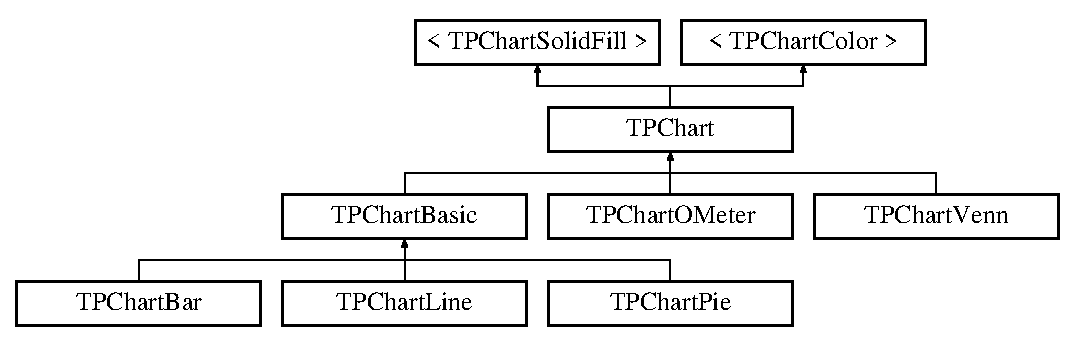
\includegraphics[height=3.5443cm]{interface_t_p_chart}
\end{center}
\end{figure}
\subsection*{Public Member Functions}
\begin{CompactItemize}
\item 
(NSMutableString $\ast$) - \hyperlink{interface_t_p_chart_0de05415b5d6de4d791a119a51468bf8}{URL}
\item 
(NSURLRequest $\ast$) - \hyperlink{interface_t_p_chart_34d673557c84b693e02cd5fe587b9c6f}{imageRequest}
\end{CompactItemize}
\subsection*{Properties}
\begin{CompactItemize}
\item 
NSSize \hyperlink{interface_t_p_chart_050f86ea651d6dee6d96cec69ff3a617}{size}
\end{CompactItemize}


\subsection{Detailed Description}
The base class of all charts. This is an abstract class. You should not instantiate it! manages the charts data and their titles 

\subsection{Member Function Documentation}
\hypertarget{interface_t_p_chart_34d673557c84b693e02cd5fe587b9c6f}{
\index{TPChart@{TPChart}!imageRequest@{imageRequest}}
\index{imageRequest@{imageRequest}!TPChart@{TPChart}}
\subsubsection[{imageRequest}]{\setlength{\rightskip}{0pt plus 5cm}- (NSURLRequest $\ast$) imageRequest }}
\label{interface_t_p_chart_34d673557c84b693e02cd5fe587b9c6f}


Returns a request for the generated Image \begin{Desc}
\item[Returns:]request for a png image \end{Desc}


Reimplemented in \hyperlink{interface_t_p_chart_line_2fa4ce27ed67bce0c2d0d2a9b41c026c}{TPChartLine}.\hypertarget{interface_t_p_chart_0de05415b5d6de4d791a119a51468bf8}{
\index{TPChart@{TPChart}!URL@{URL}}
\index{URL@{URL}!TPChart@{TPChart}}
\subsubsection[{URL}]{\setlength{\rightskip}{0pt plus 5cm}- (NSMutableString $\ast$) URL }}
\label{interface_t_p_chart_0de05415b5d6de4d791a119a51468bf8}


URL to generate the chart \begin{Desc}
\item[Returns:]the url who generates the chart \end{Desc}


\subsection{Property Documentation}
\hypertarget{interface_t_p_chart_050f86ea651d6dee6d96cec69ff3a617}{
\index{TPChart@{TPChart}!size@{size}}
\index{size@{size}!TPChart@{TPChart}}
\subsubsection[{size}]{\setlength{\rightskip}{0pt plus 5cm}- (NSSize) size\hspace{0.3cm}{\tt  \mbox{[}read, write, assign\mbox{]}}}}
\label{interface_t_p_chart_050f86ea651d6dee6d96cec69ff3a617}


Size of the chart 

The documentation for this class was generated from the following files:\begin{CompactItemize}
\item 
TPChart.h\item 
TPChart.m\end{CompactItemize}
